\chapter{Technische Grundlagen}
\label{TechnischeGrundlagen}
\section{FlexSensor}
\label{tGl_FlexSensor}
\section{Balancing}
\label{tGl_Balancing}
Das Board wird durch einen sechs Zellen Li-Po Akku gespeist. Jede einzelne Zelle hat dabei einen eigenen Innenwiderstand, welcher sich mit dem Alter verändern kann. Beim Ladevorgang entstehen somit unterschiedliche Spannungen wodurch die Zellen aus der Balance geraten.
Damit sich einzelne Zellen nicht überladen während andere leer bleiben, benötigt es einen Balancing-Vorgang um die Differenzen der Zellen auszugleichen. 
Dabei werden bei einer zu grossen Spannungsdifferenz alle Zellen auf die Spannung der niedrigsten Zelle entladen. Dabei wird in unserem Fall die überschüssige Energie über den Transistor und die Widerstände verheizt.

\section{BLDC Motor}
\label{tGl_BLDC}

Für dieses Projekt wurde der Motor OX1 2-10 zur Verfügung gestellt. Dies ist ein dreiphasen Brushless DC-Motor ohne Hallsensoren. Die gegebenen technischen Daten sind in der untenstehenden Tabelle \ref{tabBLDCdaten}) ersichtlich. 
\todo{ref neben oben ... stehend u Referenz; in der nebenstehenden Tabelle} 
Des Weiteren ist am Motor ersichtlich, dass die Erregung aus 14 Permanentmagneten besteht und somit 7 Polpaare resultieren. Der Stator besteht aus 12 Spulen, somit ist jede Phase vier Mal gewickelt.
Der Aufbau entspricht einem Aussenläufermotor, ein BLDC-Motor verhält sich aus Regelungssicht wie eine permanenterregte Synchronmaschine. In der Abbildung \ref{figAufbauBLDC} ist das Feldverhalten dargestellt.\\

\begin{figure} [H]
%	\centering
	\subfigure[Prinzip Aufbau BLDC \cite{ElAntriebe_Babiel}]{
		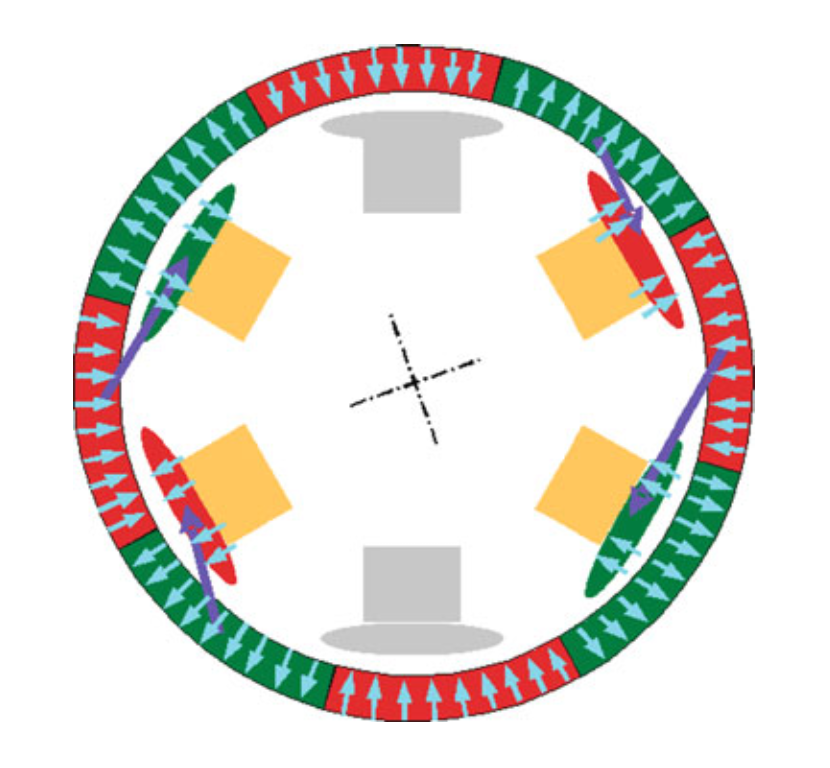
\includegraphics[width=0.45\linewidth]{images/AufbauBLDC} \label{figAufbauBLDC} 	}
	\subfigure[Sinstr][Sinusstrom mit PWM-Spannung \cite{InTech_PWM}]{ 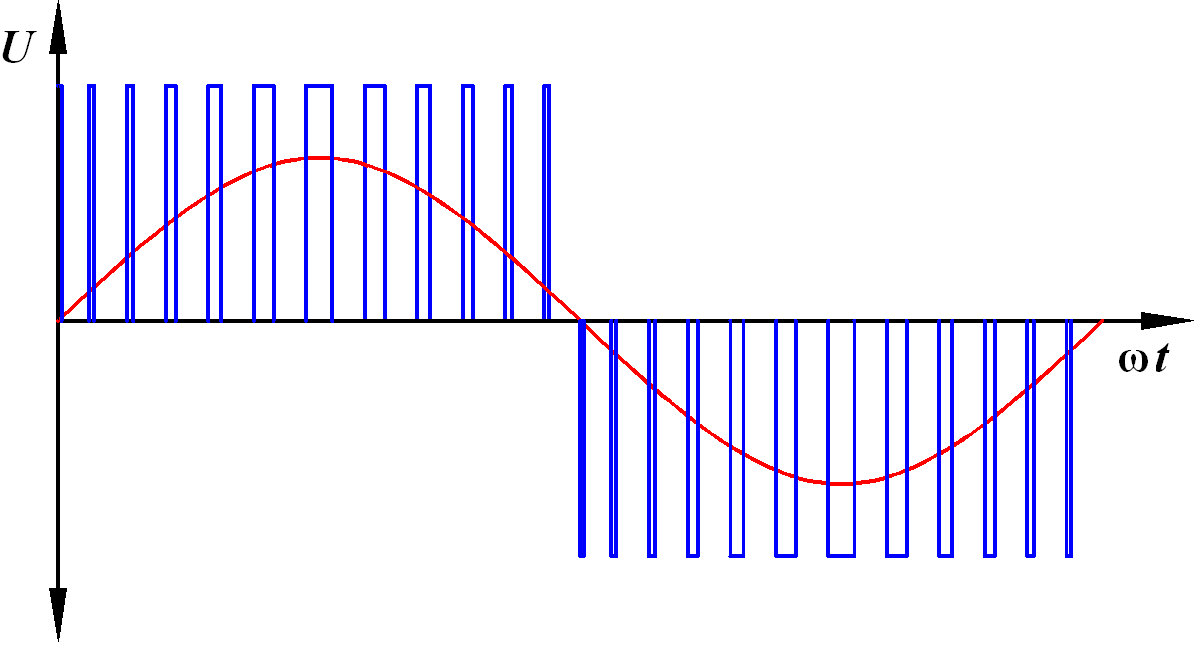
\includegraphics[width=0.5\linewidth]{images/StromBLDC} \label{figSinusstromPWM}}
	\caption[BLDC Motor]{Aufbau BLDC und PWM-Ansteuerung}
	\label{fig:BLDC}
\end{figure}

Angesteuert wird jede Phase über eine Halbbrücke. Die FOC-Regelungsweise (siehe Kapitel \ref{tGl_FOC}), setzt einen sinusförmigen Strom auf jeder Phase voraus, dies jeweils 120\(^\circ\) Phasenverschoben. \todo{ausschreiben od mit Zeichen? 120\(^\circ\) od 120 Grad?} Realisiert wird dies mittels PWM-Ansteuerung der Halbbrücken. Da der Strom bei einer L-Last das Integral der Spannung ist, lässt sich ein quasi-sinusförmiger Strom generieren. Dargestellt ist dies in der Abbildung \ref{figSinusstromPWM}.

\begin{center}
	\begin{tabular}{|c|c|}
		\hline 
		\rule[-1ex]{0pt}{2.5ex}  BLDC Motor & Werte  \\ 
		\hline 
		\rule[-1ex]{0pt}{2.5ex} Idle Current & 1.2A \\ 
		\hline 
		\rule[-1ex]{0pt}{2.5ex} Max. Current & 50A \\ 
		\hline
		\rule[-1ex]{0pt}{2.5ex} Input Volt. & 2..10 x 3.6 Lipo (25.2V) \\ 
		\hline
		\rule[-1ex]{0pt}{2.5ex} Max. Output & 1815W \\ 
		\hline
		\rule[-1ex]{0pt}{2.5ex} Max. Pull & 6700g \\ 
		\hline
		\rule[-1ex]{0pt}{2.5ex} Rated Curren & 42.5A \\ 
		\hline
		\rule[-1ex]{0pt}{2.5ex} Motor Weight & 460g \\ 
		\hline
		\rule[-1ex]{0pt}{2.5ex} Shaft & 8mm \\ 
		\hline
		\rule[-1ex]{0pt}{2.5ex} Motor dimension & \O 50 x 65mm \\ 
		\hline
		\rule[-1ex]{0pt}{2.5ex} Internal Resistance & 0.0361$\Omega$ \\ 
		\hline	
	\end{tabular} 
	\captionof{table}{BLDC Daten}
	\label{tabBLDCdaten}
\end{center}
\todo{e-Deutsch uebersetzung und Formatierung usw}
\todo{ev in Anhang??}

%\begin{figure} [H]
%	\centering
%	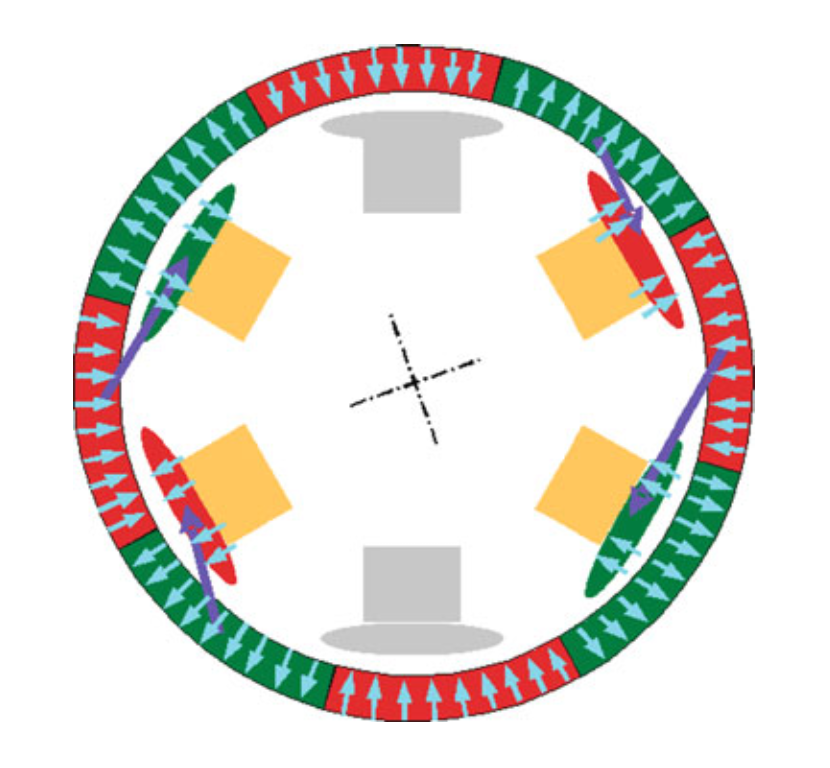
\includegraphics[width=0.4\linewidth]{images/AufbauBLDC}
%	\caption[Prinzip Aufbau]{Prinzip Aufbau}
%	\label{fig:aufbaubldc}
%\end{figure}

%\begin{figure} [H]
%	\centering
%	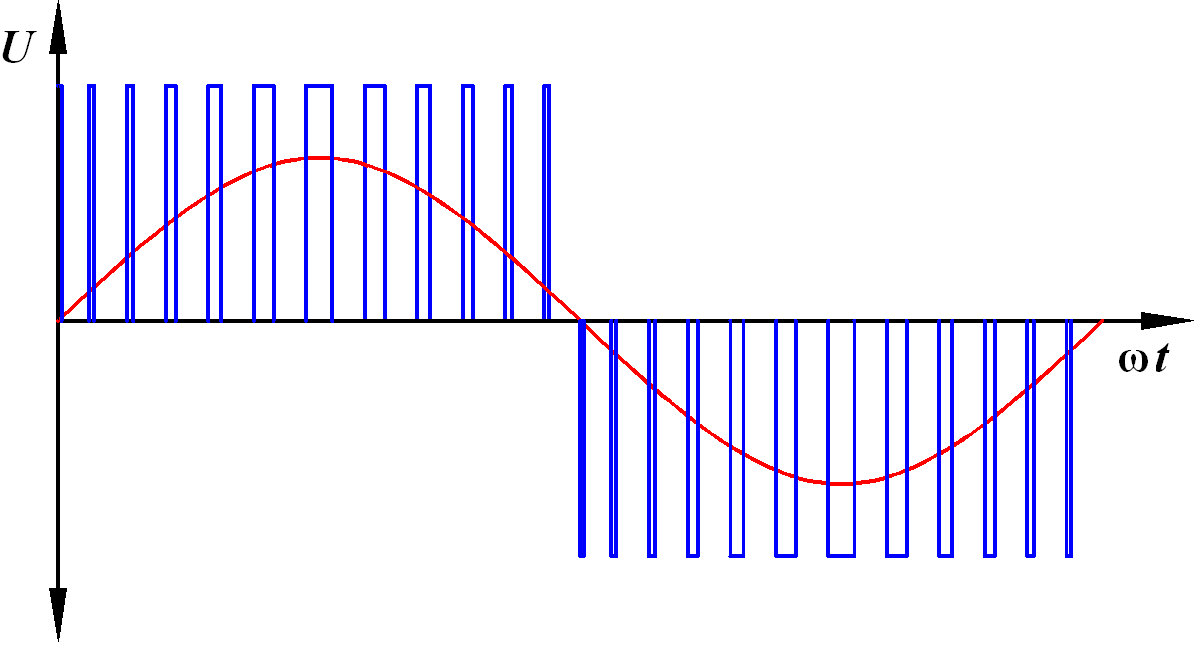
\includegraphics[width=0.5\linewidth]{images/StromBLDC}
%	\caption[Sinusstrom mit PWM Spannung]{Sinusstrom mit PWM Spannung}
%	\label{fig:strombldc}
%\end{figure}


\todo{\cite{ElAntriebe_Babiel} und korrekt zitieren...}


\section{FOC}
\label{tGl_FOC}
Einstieg...\todo{Einstieg}\\
\todo{LEserführung, Metaebene!}\\
Das Prinzip der Transformationen:
Ein kompliziertes Problem wird in ein anderes Koordinatensystem transformiert. Das transformierte Problem ist dort viel einfacher zu lösen, es ist also ein einfacheres Problem. Die leicht gefundene Lösung wird rücktransformiert, wodurch die Lösung des komplizierten Problems erhalten wird. Ein mögliches Beispiel dafür ist die Laplace-Transformierung von Differentialgleichungen. 
\\
In unserem Beispiel ist das Problem die Ansteuerung des Motors. Mit der Clarke-Transformation wird in ein statorfestes Koordinatensystem gewechselt, mit der anschliessenden Park-Transformation in ein rotorfestes. Das Problem ist nun linear und mit einem einfachen PI (oder PID) Regler lösbar. \\
Anschliessend wird die gefundene Lösung zurücktransformiert. Dabei kann die komplette Rücktransformation (inverse Park- und inverse Clarke Transformation) ausgeführt und anschliessend der Motor über eine PWM angesteuert werden, oder aber es wird nur bis ins statorfeste Koordinatensystem rücktransformiert, (inverse Park Transformation) dann wird der Motor über eine Raumvektor-PWM (SVPWM) angesteuert.


\subsection*{Clarke- und Park-Transformation}
\todo{Leserführung}
\todo{ev. subsections nummeriert?!}
\subsubsection*{Clarke-Transformation}
Die Clarke-Transformation wechselt die mehr- bzw. dreiphasigen Grössen (z.B. Phasenströme) in ein statorfestes Bezugssystem. Das kartesische Koordinatensystem ist in der komplexen Ebene. Die drei Phasenströme I$_{a}$, I$_{b}$ und I$_{c}$ werden auf zwei komplexwertige Ströme I$_{\alpha}$ und I$_{\beta}$ abgebildet. Dargestellt ist die Transformation in xxx.
%Die Transformation kann geometrisch hergeleitet werden. (xxx…)
Die mathematische Formulierung lautet:
\begin{equation}\label{ClarkeTrafo}
\left[
	\begin{array}{c}
	I_\alpha \\ 
	I_\beta
	\end{array} 
\right]
= \frac{2}{3}
\left[
	\begin{array}{ccc}
	1 & -\frac{1}{2} & -\frac 12 \\ 
	0 & \frac{\sqrt{3}}{2} & -\frac{\sqrt{3}}{2}
	\end{array} 
\right] 
\left[
	\begin{array}{c}
	I_A \\ 
	I_B \\
	I_C
	\end{array} 
\right]
\end{equation}
\todo{Abstände zwischen den Zeilen der Matrix?! ... schönere Darstellung gewünscht; Entscheid ob Multiplikationspunkt cdot dazwischen}
Die inverse Clarke-Transformation wird entsprechend durch folgende Gleichung beschrieben:
\begin{equation}\label{invClarkeTrafo}
\left[
\begin{array}{c}
	I_A \\ 
	I_B \\
	I_C
\end{array} 
\right]
= 
\left[
	\begin{array}{cc}
	1 & 0 \\
	-\frac{1}{2} & \frac{\sqrt{3}}{2} \\
	-\frac 12  & -\frac{\sqrt{3}}{2}
	\end{array} 
\right] 
\left[
	\begin{array}{c}
	I_\alpha \\ 
	I_\beta
	\end{array} 
\right]
\end{equation}


\subsubsection*{Park-Transformation}
Die Park-Transformation transformiert die Grössen I$_{\alpha}$ und I$_{\beta}$ in ein rotorfestes Bezugssystem. Dieses neue kartesische Koordinatensystem besteht aus zwei Achsen, und von aussen gesehen (ruhendes Bezugssystem) rotiert es mit der gleichen Winkelgeschwindigkeit wie der Rotor. Eine Achse wird als d-Achse (direct axis) bezeichnet, die andere als q-Achse (quadrature axis). Die d-Achse beschreibt die magnetische Flussdichte des Rotors, die q-Achse das Drehmoment des Rotors. \\
Ausgehend vom statorfesten Bezugssystem benötigt es nur noch eine Rotation, um die Grössen in das rotorfeste Bezugssystem zu transformieren. Mathematisch gesehen geschieht die Transformation also über eine Drehmatrix, dargestellt ist die Transformation in der Gleichung \ref{ParkTrafo}. 
\begin{equation}\label{ParkTrafo}
\left[
	\begin{array}{c}
	I_d \\ 
	I_q
	\end{array} 
\right]
= 
\left[
	\begin{array}{cc}
	\cos (\theta) & \sin(\theta) \\
	-\sin(\theta)  & \cos(\theta)
	\end{array} 
\right] 
\left[
	\begin{array}{c}
	I_\alpha \\ 
	I_\beta
	\end{array} 
\right]
\end{equation}

Die inverse Park-Transformation wird entsprechend durch folgende Gleichung beschrieben:
\begin{equation}\label{invParkTrafo}
\left[
	\begin{array}{c}	
	I_\alpha \\ 
	I_\beta
	\end{array} 
\right]
= 
\left[
	\begin{array}{cc}
	\cos (\theta) & -\sin(\theta) \\
	\sin(\theta)  & \cos(\theta)
	\end{array} 
\right] 
\left[
	\begin{array}{c}
	I_d \\ 
	I_q
	\end{array} 
\right]
\end{equation}

\subsubsection*{d/q-Transformation} 
Die Clarke- und Park-Transformation kann auch in einem Schritt durchgeführt werden, je nach Quelle wird diese dann auch Park-Transformation oder d/q-Transformation genannt. [xxx Quelle!] 
Die mathematische Formulierung lautet:
\begin{equation}\label{dqTrafo}
\left[
	\begin{array}{c}
	I_d \\ 
	I_q
	\end{array} 
\right]
= \frac{2}{3}
\left[
	\begin{array}{ccc}
	\cos (\theta) & \cos (\theta-\frac{2\pi}{3} & \cos (\theta-\frac{4\pi}{3} \\ 
	-\sin (\theta) & -\sin (\theta-\frac{2\pi}{3} & -\sin (\theta-\frac{4\pi}{3}
	\end{array} 
\right] 
\left[
	\begin{array}{c}
	I_A \\ 
	I_B \\
	I_C
	\end{array} 
\right]
\end{equation}

Die inverse d/q-Transformation lautet:
\begin{equation}\label{invdqTrafo}
\left[
	\begin{array}{c}
	I_A \\ 
	I_B \\
	I_C
	\end{array} 
\right]
=
\left[
	\begin{array}{cc}
	\cos (\theta) & -\sin (\theta) \\
	\cos (\theta-\frac{2\pi}{3} & -\sin (\theta-\frac{2\pi}{3} \\
	\cos (\theta-\frac{4\pi}{3} & -\sin (\theta-\frac{4\pi}{3} 
	\end{array} 
\right] 
\left[
	\begin{array}{c}
	I_d \\ 
	I_q
	\end{array} 
\right]
\end{equation}


\subsection*{PI-Regler}
Ein PI-Regler ist ein Regler mit einem Proportional- (P) und einem Integral- (I) Glied. Dies sind elementare Glieder der Regelungstechnik. Das P-Glied entspricht einer Multiplikation des Eingangs mit einer zeitunabhängigen Konstanten, das P-Glied einer Integration des Eingangs. 
\\\\
Die Regelung mit einem PI-Regler geschieht im rotorfesten Bezugssystem, Gegenstand der Regelung sind die Flussdichte des Motors (d-Komponente) und das Drehmoment (q-Komponente). Bei einem permanenterregten Motor ist diese Regelung vereinfacht. In der Abb.xxx ist ersichtlich, dass die d-Achse in Richtung des Permanentmagneten zeigt. Das grösste resultierende Moment wird erreicht, wenn die resultierende Flussdichte im Stator um 90\(^\circ\) zur zeitlich konstanten Flussdichte des Rotors verschoben ist. Dies zeigt also genau in Richtung der q-Achse. Die resultierende Flussdichte liegt also auf der q-Achse und hat deshalb keinen d-Anteil. Der Sollwert der d-Komponente wird also null. Das Drehmoment kann somit direkt über die q-Komponente geregelt werden. 

\todo{Ev. Begründung warum PI Regler, ohne D, Iteil grösser… träges system, d für schenlle änderungen}




\subsection*{Nonlinear Observer}
Die Park-Transformation benötigt die momentane Lage des Rotors. Da der vorgegebene Motor nicht über integrierte Sensoren (wie beispielsweise Hall-Sonden) verfügt, die Ansteuerung also sensorlos erfolgt, muss der Winkel der Rotorlage auf einem anderen Weg herausgefunden werden. Dazu gibt es verschiedene Varianten. 
Ev. Tabelle mit Variante, Pro, Contra; Erläuerungen \todo{Tabelle od Ausformulierung der Gründe für diese Variante}
Im Team wurde entschieden, die Winkelschätzung über einen nichtlinearen Beobachter, nonlinear observer genannt, vorzunehmen. (Formulierung! Und Begründung…) Dazu wird ein mathematisches Modell des Motors erstellt. Zudem werden die Phasenströme gemessen. Mit diesen Informationen wird eine Simulation des Motors durchgeführt, und aufgrund der aktuellen Parameter wird die Position ermittelt. Dies funktioniert, da aufgrund der Phasenströme auf die Lage des Motors rückgeschlossen werden kann. Beschrieben wird dieses Verfahren in xxx [Quelle IEEE-Paper].
\todo{Quelle nonlinear Observer}


\section{FET, H-Brücke}
\label{tGl_HBrugg}
\section{Funkübertragung}
\label{tGl_RF}
